\documentclass[hyperref,UTF8,10pt]{beamer}
\usepackage[heading=true]{ctex}
% \usepackage[utf8]{inputenc}
\usepackage{fontspec}
\usepackage{comment}
\usepackage{minted}
\setmonofont{Consolas}
\setsansfont{Microsoft YaHei}
\setCJKmainfont{Microsoft YaHei}
\usefonttheme{professionalfonts}
\usepackage{graphicx}
\graphicspath{image/} % storage figure in a sub-folder
\usepackage{tjcolor}
\hypersetup{CJKbookmarks=true}
\usepackage{url}
\usepackage{amsmath}
\usepackage{amssymb}
\usepackage{amsthm}
\usepackage{booktabs} % for much better looking tables
\usepackage{array} % for better arrays (eg matrices) in maths
%\usepackage{paralist} % very flexible & customisable lists (eg. enumerate/itemize, etc.)
\usepackage{verbatim} % adds environment for commenting out blocks of text & for better verbatim
\usepackage{subfigure} % make it possible to include more than one captioned figure/table in a single float
% These packages are all incorporated in the memoir class to one degree or another...
%\usepackage{threeparttable}
% \usepackage{cases} %equation set
% \usepackage{multirow} %use table
% \usepackage{enumerate}
\usepackage{algorithm}
\usepackage{algpseudocode}
\usepackage{xcolor}
\usepackage{bm}
%\usepackage{capt-of}
\setcounter{tocdepth}{1}%只显示section,不显示subsection
\usepackage{listings}
\numberwithin{equation}{section} %按节编号
% \usepackage[colorlinks=true]{hyperref}
\newcommand{\degree}{^\circ}
\newcommand{\ud}{\,\mathrm{d}}

\title{GitHub详解}
% \subtitle{English Title}
\author[Peter YU]
{
汇报人:余周炜
}
\institute[Tongji CSGI]{同济大学\quad 测绘与地理信息学院}
\date{\today} %Activate to display a given date or no date (if empty),
% otherwise the current date is printed

\begin{document}
%%%%%%%%%% 定理类环境的定义 %%%%%%%%%%
%% 必须在导入中文环境之后
\newcommand{\redstress}[1]{{\color{red}{#1}}}

%----------------------------------------------------------------------
% Title frame
\begin{frame}
\maketitle
\end{frame}

\section{Git简介}

\begin{frame}{Git是什么}
    Git是一个开源的分布式版本控制系统,它在软件开发中最终源代码的改变,并允许多人协作。最初由Linus Trovalds开发,可以有效、高速地处理项目版本管理。

\end{frame}

\begin{frame}{什么叫版本控制系统?}

比方说你用Word写论文,想删除一个段落,又怕找不回来怎么办?

有办法,先将文件"另存为..."一个新的Word文件,改到一定程度,再"另存为..."一个新的文件。更要命的还需要别人帮你写。

于是你想,如果有一个软件,不但能自动帮我记录每次文件的改动,还可以让同事协作编辑,这样就不用自己管理一堆类似的文件了,也不需要把文件传来传去。如果想查看某次改动,只需要在软件里瞄一眼就可以,岂不是很方便?


这个软件用起来就应该像这个样子,能记录每次文件的改动:
\begin{figure}
\centering
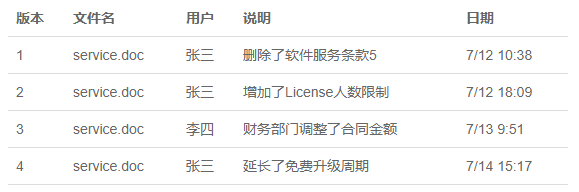
\includegraphics[width=0.85\textwidth]{VerControl.PNG}
\caption{版本控制系统}
\end{figure}

\end{frame}


\begin{frame}{创建版本库}
\begin{enumerate}
\item 创建一个空目录。
\item 通过\emph{git init}命令把这个目录变成Git可以管理的仓库,当前目录下多了一个\emph{.git}目录。
\end{enumerate}
\end{frame}


\begin{frame}{提交}
将一个文件修改好后,两步提交:
\begin{enumerate}
\item git add <file>
\item git commit -m <message>
\end{enumerate}

注:在Github Desktop客户端里面一步到位,点击Commit to master将所有更改提交。
\end{frame}

\begin{frame}{工作区和版本库}

\begin{description}
\item[工作区(Working Directory)] 就是你在电脑里能看到的目录。
\item[版本库(Repository)] 工作区的隐藏目录\emph{.git}。 
\end{description}

Git的版本库里存了很多东西,其中最重要的就是称为stage(或者叫index)的暂存区,还有Git为我们自动创建的第一个分支master,以及指向master的一个指针叫HEAD。

\begin{figure}
\centering
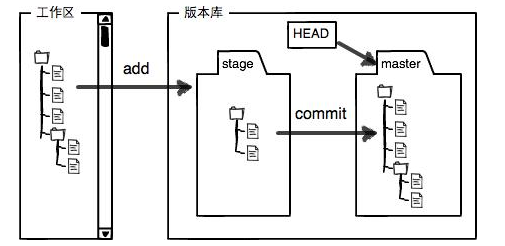
\includegraphics[width=0.85\textwidth]{ku.PNG}
\caption{工作区和版本库}
\end{figure}

\begin{figure}
\centering
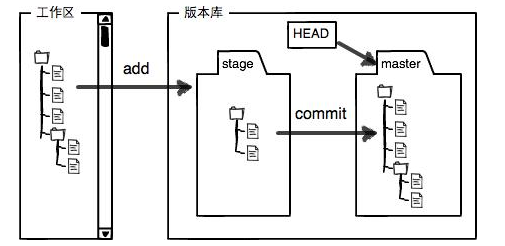
\includegraphics[width=0.85\textwidth]{ku.PNG}
\caption{工作区和版本库}
\end{figure}

\end{frame}

\begin{frame}{暂存区和分支}
    前面讲了我们把文件往Git版本库里添加的时候,是分两步执行的:

    第一步是用git add把文件添加进去,实际上就是把文件修改添加到暂存区;
    
    第二步是用git commit提交更改,实际上就是把暂存区的所有内容提交到当前分支。
\begin{columns}
\begin{column}{.5\textwidth}
    \begin{figure}
    \centering
    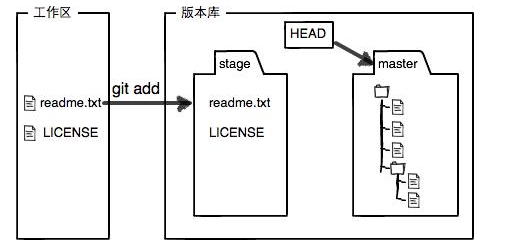
\includegraphics[width=\textwidth]{add.PNG}
    \caption{git add}
    \end{figure}
\end{column}
\begin{column}{.5\textwidth}
    \begin{figure}
    \centering
    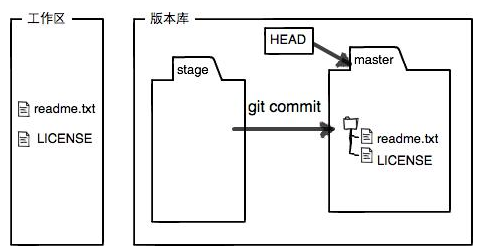
\includegraphics[width=\textwidth]{commit.PNG}
    \caption{git commit}
    \end{figure}
\end{column}
\end{columns}

\end{frame}


\section{远程仓库Github}

\begin{frame}{简介}
GitHub是一个面向开源及私有软件项目的托管平台,因为只支持git 作为唯一的版本库格式进行托管,故名GitHub。
\end{frame}

\begin{frame}{添加远程库}

首先,登陆GitHub,然后,在右上角找到“Create a new repo”按钮,创建一个新的仓库

在Repository name填入learngit,其他保持默认设置,点击“Create repository”按钮,就成功地创建了一个新的Git仓库

然后通过点击Clone or download,Open in Desktop来将远程库克隆到本地。

默认,git 本地库的主分支叫master,远程库叫origin fetch(取来)到本地。

分支管理参见
https://www.liaoxuefeng.com/wiki\\
/896043488029600/896954848507552
\end{frame}


\begin{frame}{fork别人的仓库}
\begin{figure}
\centering
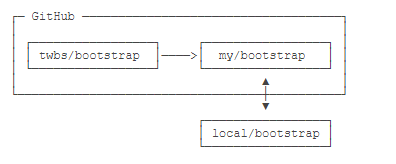
\includegraphics[width=0.85\textwidth]{clone.PNG}
\caption{fork流程}
\end{figure}

首先,点击你需要的库,然后点击fork叉到你的远程库,随后再clone到本地。
\end{frame}

\begin{frame}{关系图}
\begin{figure}
\centering
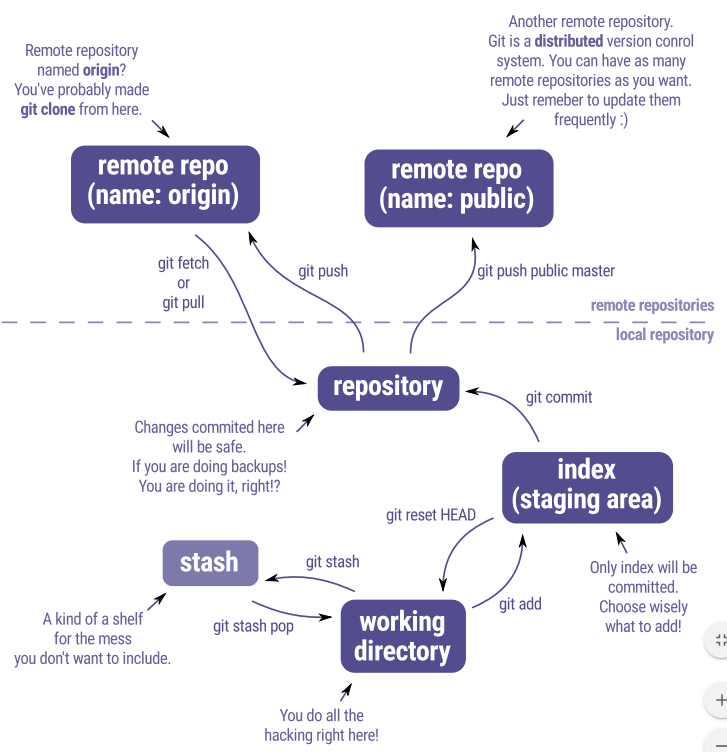
\includegraphics[height=\textheight]{rela.PNG}
\caption{Git Relation}
\end{figure}
\end{frame}

\section{小组合作}
\begin{frame}

Github多人协作开发有三种方式:
\begin{itemize}
\item Fork方式。开发者 fork 自己生成一个独立的分支,跟主分支完全独立,pull代码后,项目维护者可根据代码质量决定是否merge代码
\item 组织。组织的所有者可以针对不同的代码仓库建立不同访问权限的团队。
\item 合作者。代码仓库的所有者可以为单个仓库增加具备只读或者读写权限的协作者。

合作者方式比较实用,也很方便,新建一个Repository,完毕之后,进入Repository的Settings,然后在Manage Collaborators里就可以管理合作者了。
\end{itemize}
\end{frame}

\end{document}
